\section{Counters}\label{sec:counters}
As a first step towards accomplishing our research vision, let's begin with a
\emph{simple} CRDT with \emph{simple} operations and a \emph{simple} invariant
language: PN-Counters and linear equations and inequalities.

Recall that a \emph{G-Counter} CRDT is an increment-only counter
\cite{shapiro2011comprehensive}. A state-based G-Counter distributed across $n$
machines $1, 2, \ldots, n$ can be implemented as an $n$-tuple $(x_1, x_2,
\ldots, x_n)$ of natural numbers. The \emph{increment($k$) method} at machine
$i$ increments $x_i$ by $k$; the \emph{query method} returns the sum of the
tuple $\sum_{i=1}^n x_i$; and the \emph{merge method} computes the pairwise max
of two $n$-tuples.

A \emph{PN-Counter} CRDT is a counter which supports increments and decrements
and can be implemented as a pair $(p, n)$ of two G-Counters
\cite{shapiro2011comprehensive}. increment($x$) increments $p$ by $x$;
decrement($x$) increments $n$ by $x$; query returns $p - n$; and merge performs
a pairwise merge of $p$ and $n$.

Our \emph{invariant language} is formed from \emph{linear equations} (e.g. $x =
0$, $2x = y$, $-x + 42y - 2z = 16$) and \emph{inequalities} (e.g. $x > 0$, $2x
\leq y$, $-x + 42y - 2z \neq 16$) connected with the boolean connectives
\emph{and} ($\land$), \emph{or} ($\lor$), and \emph{not} ($\lnot$) (e.g.
$\lnot((\lnot(x < 0) \lor 2x = y) \land -x + 42y - 2z \geq 16)$).

A \emph{transaction} chooses a subset of variables and decrements or increments
each by a constant amount. For example, a transaction may increment $x$ by 1,
decrement $y$ by 42, and increment $z$ by 100.

Given a set of transactions and an invariant, we want to determine whether the
transactions are \iconfluent{} with respect to the invariant. For example, the
transaction that \emph{increments} $x$ by 1 is \iconfluent{} with respect to
the invariant $x > 0$, but the transaction that \emph{decrements} $x$ by 1 is
not, as shown in \figref{decrement}.

\begin{figure}[h]
  \centering
  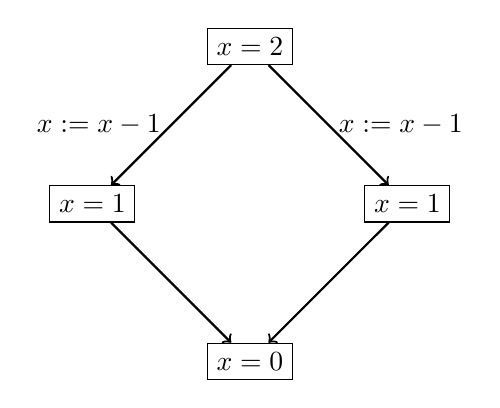
\begin{tikzpicture}
    \node[draw] (start)  at (2, 4) {$x=2$};
    \node[draw] (left)   at (0, 2) {$x=1$};
    \node[draw] (right)  at (4, 2) {$x=1$};
    \node[draw] (merged) at (2, 0) {$x=0$};

    \draw[thick, ->] (start) to node[left]  {$x := x - 1$} (left);
    \draw[thick, ->] (start) to node[right] {$x := x - 1$} (right);
    \draw[thick, ->] (left)  to (merged);
    \draw[thick, ->] (right) to (merged);
  \end{tikzpicture}
  \caption{
    A counterexample showing transaction $x := x - 1$ is not invariant
    confluent with respect to the invariant $x > 0$. The top, left, and right
    states satisfy the invariant, but the bottom state does not.
  }
  \label{fig:decrement}
\end{figure}
